\documentclass[english]{article}
\usepackage[T1]{fontenc}
\usepackage[latin9]{inputenc}
\usepackage{geometry}
\geometry{verbose,tmargin=2cm,bmargin=2cm,lmargin=2cm,rmargin=2cm}
\usepackage{float}
\usepackage{amsmath}
\usepackage{amssymb}
\usepackage{graphicx}
\usepackage{setspace}
\usepackage[authoryear]{natbib}

\makeatletter
%%%%%%%%%%%%%%%%%%%%%%%%%%%%%% User specified LaTeX commands.
\usepackage{ae,lmodern}
\usepackage{graphicx}
\usepackage{lineno}
\usepackage{authblk}
\date{}
\DeclareMathOperator\erf{erf}

\makeatother

\usepackage{babel}
\begin{document}
\textbf{Supporting Information} for \textit{Local intraspecific aggregation
in phytoplankton model communities: spatial scales of occurrence and
implications for coexistence}\emph{ }by C. Picoche, W.R. Young \&
F. Barraquand.

\renewcommand\thesection{S\arabic{section}}
\setcounter{section}{0}
\renewcommand\thefigure{S\arabic{figure}}
\setcounter{figure}{0}
\renewcommand\theequation{S\arabic{equation}}
\setcounter{equation}{0}

\section{Derivation of the turbulent map}

We show here how to derive a discrete-time map for turbulence from
the continuous-time formula. We consider that the velocity field $\textbf{u}^{T}=(u_{x}\,u_{y}\,u_{z})$
at position $\mathbf{x}^{T}=(x,\,y,\,z)$ alternates between the three
dimensions during a period $\tau$, so that:

\begin{equation}
\textbf{u}^{T}(\textbf{x},t)=\begin{cases}
\begin{array}{cc}
\left(Ucos(ky+\phi),0,0\right) & \text{for }n\tau\leq t<(n+\frac{1}{3})\tau\\
\left(0,Ucos(kz+\theta),0\right) & \text{for }(n+\frac{1}{3})\tau\leq t<(n+\frac{2}{3})\tau\\
\left(0,0,Ucos(kx+\psi)\right) & \text{for }(n+\frac{2}{3})\tau\leq t<(n+1)\tau
\end{array}\end{cases}\label{eq:pierrehumber_continuous_time}
\end{equation}

The discrete-time map can be obtained by computing the displacement
over a period, between $t=n\tau$ and $t+1=(n+1)\tau$, with $\textbf{x}(t+1)=\textbf{x}(t)+\textbf{\ensuremath{\int_{n\tau}^{\left(n+1\right)\tau}}u}(\textbf{x},t)dt$,
and knowing the initial position $\mathbf{x}(t)$. This can be solved
in three steps (eq. \ref{eq:step1_pierrehumbert}, \ref{eq:step2_pierrehumbert}
and \ref{eq:step3_pierrehumbert}).

\begin{equation}
\begin{cases}
\begin{array}{cc}
x(t+\tau/3)= & x(t)+\frac{U\tau}{3}cos(ky(t)+\phi)\\
y(t+\tau/3)= & y(t)\\
z(t+\tau/3)= & z(t)
\end{array}\end{cases}\label{eq:step1_pierrehumbert}
\end{equation}

\begin{equation}
\begin{cases}
\begin{array}{cc}
x(t+2\tau/3)= & x(t+\tau/3)\\
y(t+2\tau/3)= & y(t)+\frac{U\tau}{3}cos(kz(t)+\phi)\\
z(t+2\tau/3)= & z(t)
\end{array}\end{cases}\label{eq:step2_pierrehumbert}
\end{equation}

\begin{equation}
\begin{cases}
\begin{array}{cc}
x(t+\tau)= & x(t+\tau/3)\\
y(t+\tau)= & y(t+\tau/3)\\
z(t+\tau)= & y(t)+\frac{U\tau}{3}cos(kx(t+\tau)+\phi)
\end{array}\end{cases}\label{eq:step3_pierrehumbert}
\end{equation}

In the third step, we need $z$ to be a function of $x(t+\tau)$,
not $x(t)$, so that the volume is conserved (the determinant of the
Jacobian matrix is equal to 1).

\section{Characteristics of standard spatial point processes}

In order to familiarize the reader with spatial process metrics, we
present here the analytical formulas and corresponding figures (Fig.
\ref{fig:Example-Poisson} and \ref{fig:Example-Thomas}) for the
pair correlation function, Ripley's $K$-function and dominance index
for standard point processes. We focus on the uniform distribution,
i.e. the Poisson point process, and a clustered distribution, the
Thomas point process. The Thomas point process is the result of a
two-stage mechanism: a Poisson point process generates ``parent points''
around which ``daughter points'' are scattered, their location following
a Gaussian distribution centered on the parent location, with standard
deviation $\sigma$. The numbers of parents and daughters per parent
follow two Poisson distributions with mean $N_{p}$ and $N_{d}$ respectively.

\subsection{Pair correlation function}

In the case of a Poisson point process,

\begin{equation}
\forall r\geq0\text{, }g_{ii}(r)=1
\end{equation}

For a Thomas point process, the expected value of the pcf is

\begin{equation}
g_{ii}(r)=1+\frac{1}{C_{p}}\frac{1}{\left(4\pi\sigma^{2}\right)^{3/2}}e^{-\left(\frac{r^{2}}{4\sigma^{2}}\right)}
\end{equation}

where $C_{p}=N_{p}/V$ is the concentration/intensity of the parent
process in the volume $V$.\\

More generally, for a random superposition of stationary point processes
with marks (species) $i$ and $j$, $\forall i,j,r\geq0\text{, }g_{ij}(r)=1$
\citep[ p. 326, eq. 5.3.13]{illian2008statistical}.

\subsection{Ripley's $K$-function}

In the case of a Poisson point process,

\begin{equation}
\forall r\geq0\text{, }K_{ii}(r)=\frac{4}{3}\pi r^{3}\label{eq:k_poisson}
\end{equation}

For a Thomas point process, 

\begin{equation}
K_{ii}(r)=\frac{4}{3}\pi r^{3}+\frac{1}{C_{p}\sigma\sqrt{\pi}}\left(\sigma\sqrt{\pi}\erf\left(\frac{r}{2\sigma}\right)-re^{-\left(\frac{r}{2\sigma}\right)^{2}}\right)\label{eq:k_thomas}
\end{equation}

More generally, for a random superposition of stationary point processes,
$K_{ij}(r)=\frac{4}{3}\pi r^{3}$ \citep[p. 324, eq. 5.3.5]{illian2008statistical}.

\subsection{Dominance index}

In the Poisson point process, $K_{ii}(r)=K_{ij}(r)$, which means
that the dominance index can be reduced to ratios of concentrations:

\begin{equation}
D_{i}(r)=\frac{C_{i}}{\sum_{j=1}^{S}C_{j}}
\end{equation}

In the Thomas process, using eq. \ref{eq:k_thomas}, 

\begin{equation}
D_{i}(r)=\frac{C_{i}\left(\frac{4}{3}\pi r^{3}+\frac{F(r)}{C_{p,i}}\right)}{C_{i}\frac{F(r)}{C_{p,i}}+\sum_{j}C_{j}\frac{4}{3}\pi r^{3}}
\end{equation}

with $F(r)=\frac{1}{\sigma\sqrt{\pi}}\left(\sigma\sqrt{\pi}\erf\left(\frac{r}{2\sigma}\right)-re^{-\left(\frac{r}{2\sigma}\right)^{2}}\right)$.

\begin{figure}[H]
\begin{centering}
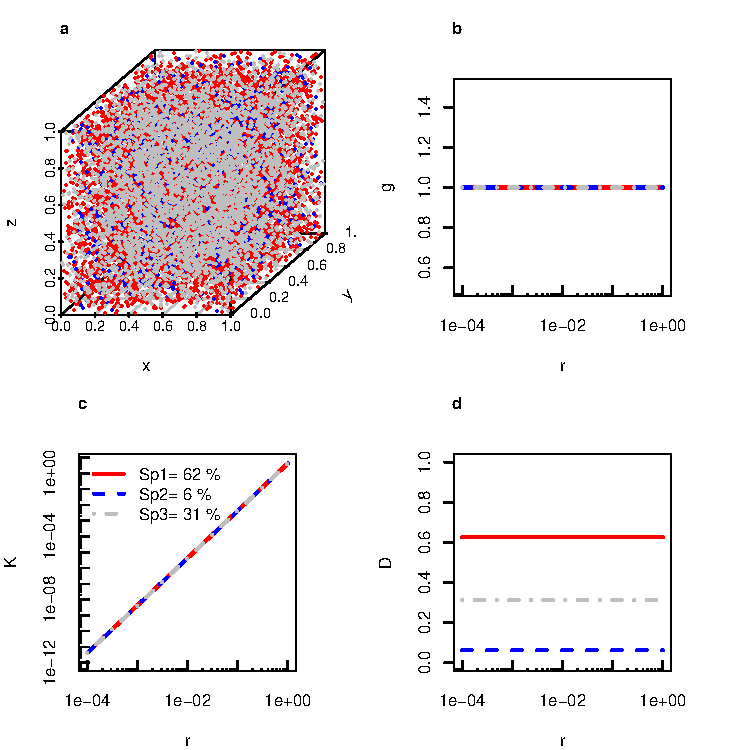
\includegraphics[width=1\textwidth]{../code/figure/example_Poisson_distribution}
\par\end{centering}
\caption{Example of spatial distribution (a) and theoretical pair correlation
function (b), Ripley's $K$-function (c) and dominance index (d) for
a Poisson point process in a 3-species community with different intensities
(10000 cm$^{-3}$, 1000 cm$^{-3}$, 5000 cm$^{-3}$). \label{fig:Example-Poisson}}

\end{figure}

\begin{figure}[H]
\begin{centering}
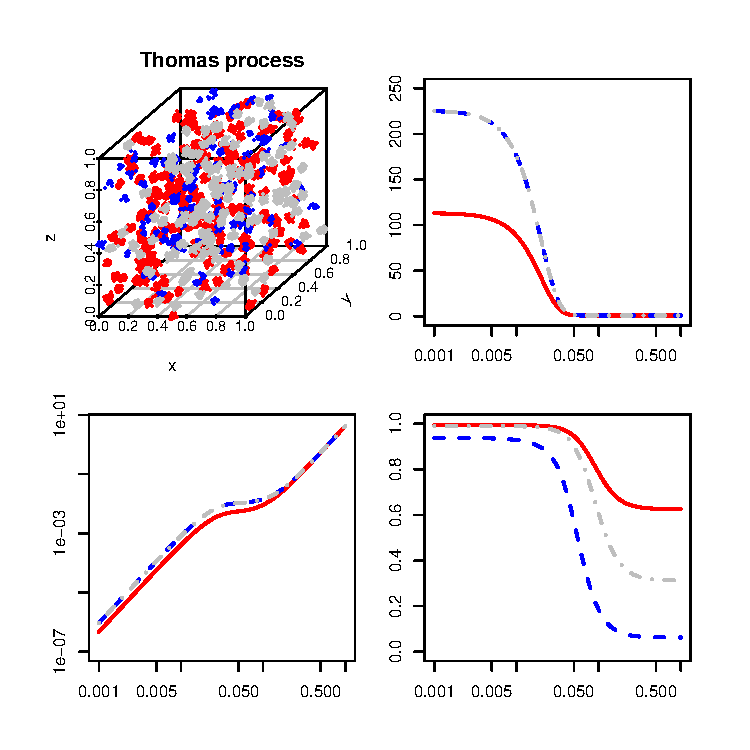
\includegraphics[width=0.75\textwidth]{../code/figure/example_Thomas_distribution}
\par\end{centering}
\caption{Example of spatial distribution (a) and theoretical pair correlation
function (b), Ripley's $K$-function (c) and dominance index (d) for
a Thomas point process in 3-species community with different parent
intensities (200 cm$^{-3}$, 100 cm$^{-3}$, 100 cm$^{-3}$), and
different children per parent intensities (50, 10, 50), with $\sigma=0.01$.\label{fig:Example-Thomas}}
\end{figure}


\section{Theoretical behaviour of the dominance index in the BBM}

With the theoretical formula for the dominance index in the Brownian
Bug Model, we can show the progressive clustering of particles with
time when advection is absent. Even after a short period of time,
the dominance index without advection is larger than with advection,
the difference being much more pronounced for larger cells. 

\begin{figure}[H]
\begin{centering}
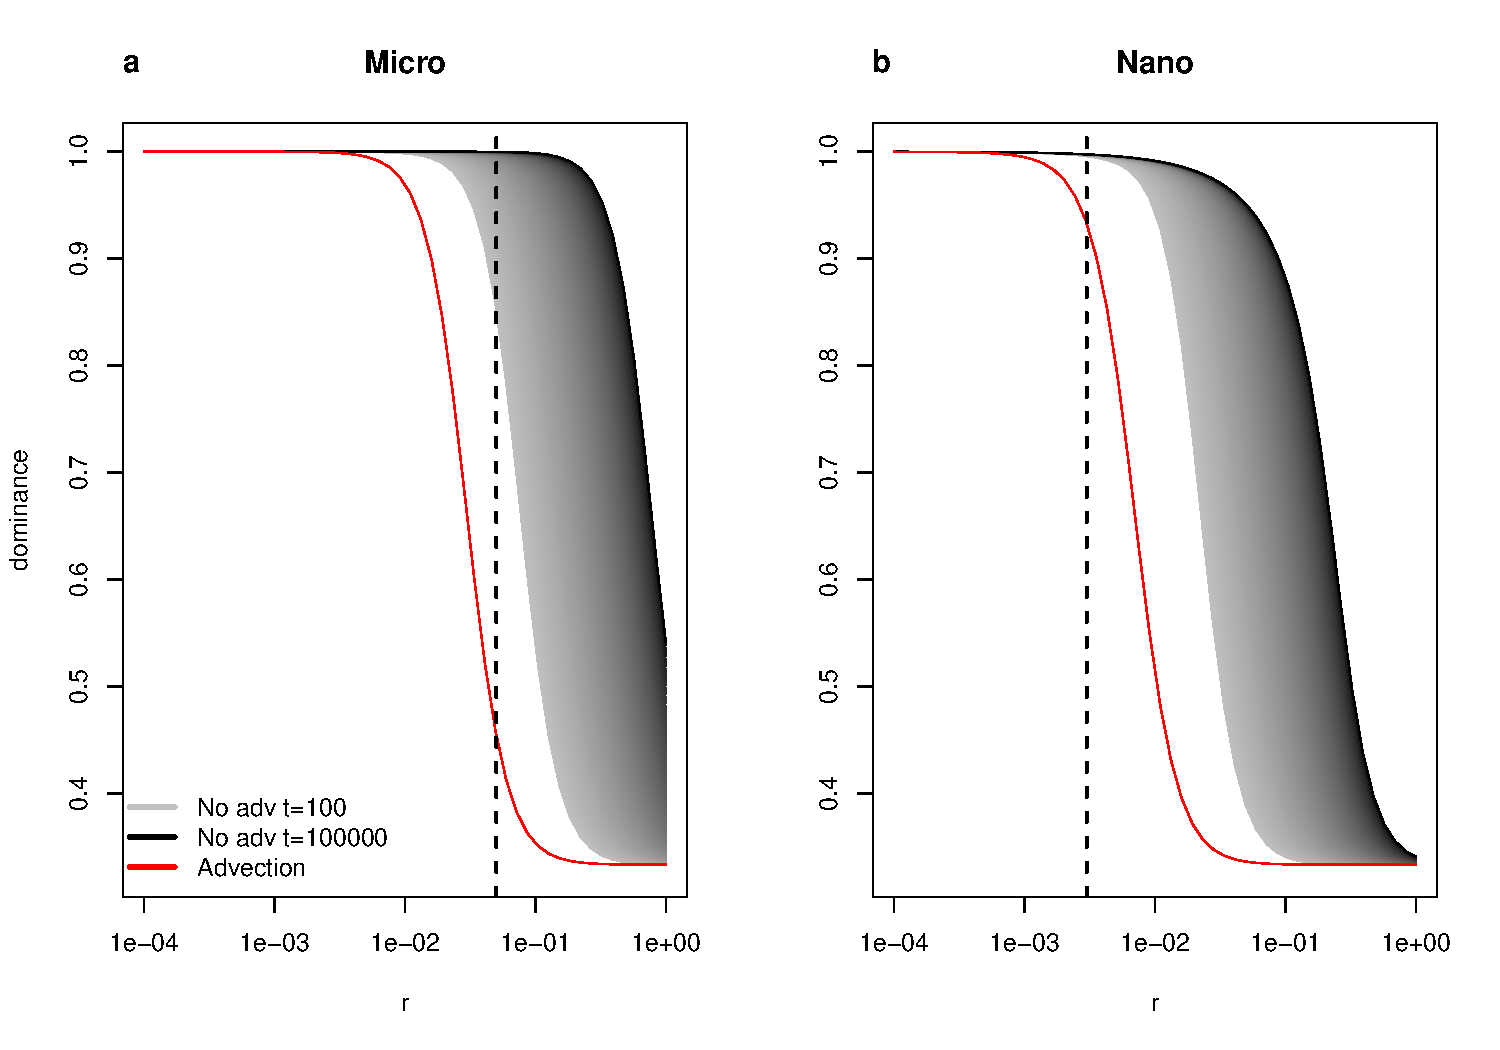
\includegraphics[width=0.8\textwidth]{../code/figure/theory_dominance}
\par\end{centering}
\caption{Theoretical dominance indices as a function of the distance (in cm)
from a particle of a given species, for a microphytoplankton (a) and
nanophytoplankton (b) 3-species community with an even abundance distribution,
with (red line) and without (grey to black lines, with darker lines
for longer duration) advection. The vertical dashed line corresponds
to the distance threshold for interaction. \label{fig:Theoretical-dom}}

\end{figure}


\section{Computation of the pair correlation function and Ripley's function}

The algorithm for the pcf computation was mostly taken from the function
\verb|pcf3est| in spatstat 2.2-0 \citep{baddeley_spatstat} and adapted
to the interspecific pcf (i.e., pcf for marked point processes).

Schematically, $g_{ij}(r)$ is estimated via the use of the Epanechnikov
kernel $\kappa_{E}$ with bandwidth $\delta$.

\begin{equation}
\begin{array}{ccc}
\hat{g}_{ij}(r) & = & \frac{1}{\hat{C_{i}}}\frac{1}{\hat{C_{j}}}\frac{1}{4\pi r^{2}}\sum_{_{i}}\sum_{j}\kappa_{E}(r-||x_{i}-x_{j}||)w(x_{i},x_{j})\end{array}\label{eq:pcf_estimate}
\end{equation}

where $w(x_{i},x_{j})$ is the Ohser translation correction estimator
\citep{ohser_estimators_1983} and the kernel is defined as follow.

\begin{equation}
\kappa_{E}(x)=\begin{cases}
\frac{3}{4\delta}\left(1-\frac{x^{2}}{\delta^{2}}\right) & \text{for }-\delta\leq x\leq\delta\\
0 & \text{otherwise}
\end{cases}
\end{equation}

The estimate $\hat{g}_{ij}(r)$ is therefore very sensitive to the
bandwidth: if it is too small, the estimate is noisy and may even
be missing several pairs of points; if it is too large, the smoothing
might be so important that values are strongly underestimated. In
spatstat 2.2-0 \citep{baddeley_spatstat}, the bandwidth default value
is $\delta=0.26C^{-1/3}$. The pcf computation function was first
tested on standard distributions (with the default bandwidth), then
on the Brownian Bug Model (with different bandwidths, see below). 

\medskip{}

Estimates of the Ripley's $K$-function were also performed with the
Ohser translation correction estimator  but did not require any kernel
smoothing.

\subsection{Standard point processes}

\begin{figure}[H]
\begin{centering}
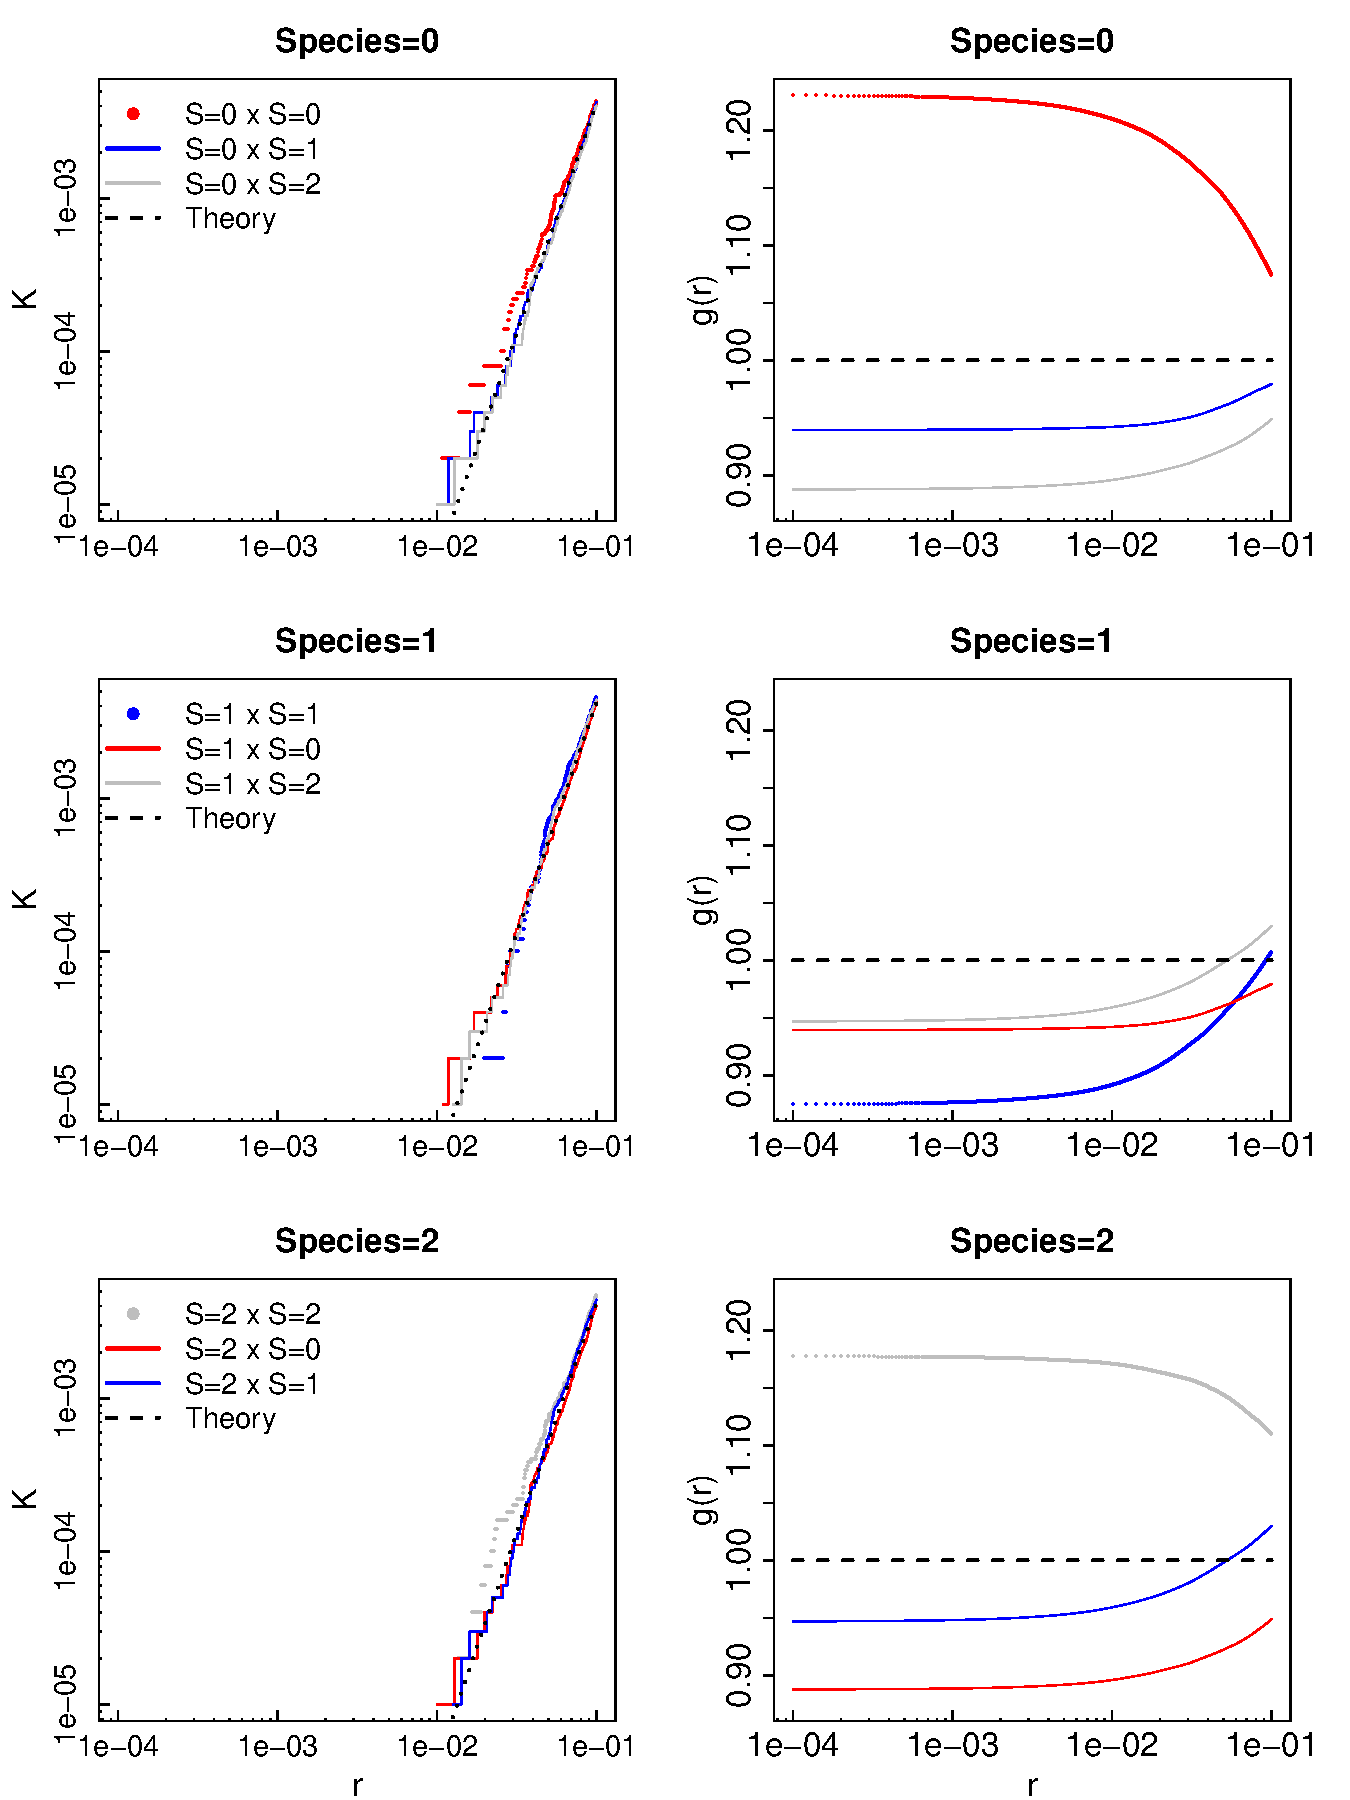
\includegraphics[height=0.85\textheight]{../code/figure/K_PCF_Poisson}
\par\end{centering}
\caption{Intra- and inter-specific Ripley's $K$-function and pair correlation
function values as a function of distance (in cm) for 3 species following
a Poisson process with intensity 10 cm$^{-3}$, in a volume of 1000
cm$^{3}$. Values computed from our simulations (circles and solid
lines for intra- and interspecific values, respectively) are compared
with theoretical formula (dotted lines). Note that theoretical values
are the same for intra and interspecific moments for the Poisson distribution.
Colors correspond to the different species (red for species 0, blue
for species 1, black for species 2). }
\end{figure}

\begin{figure}[H]
\begin{centering}
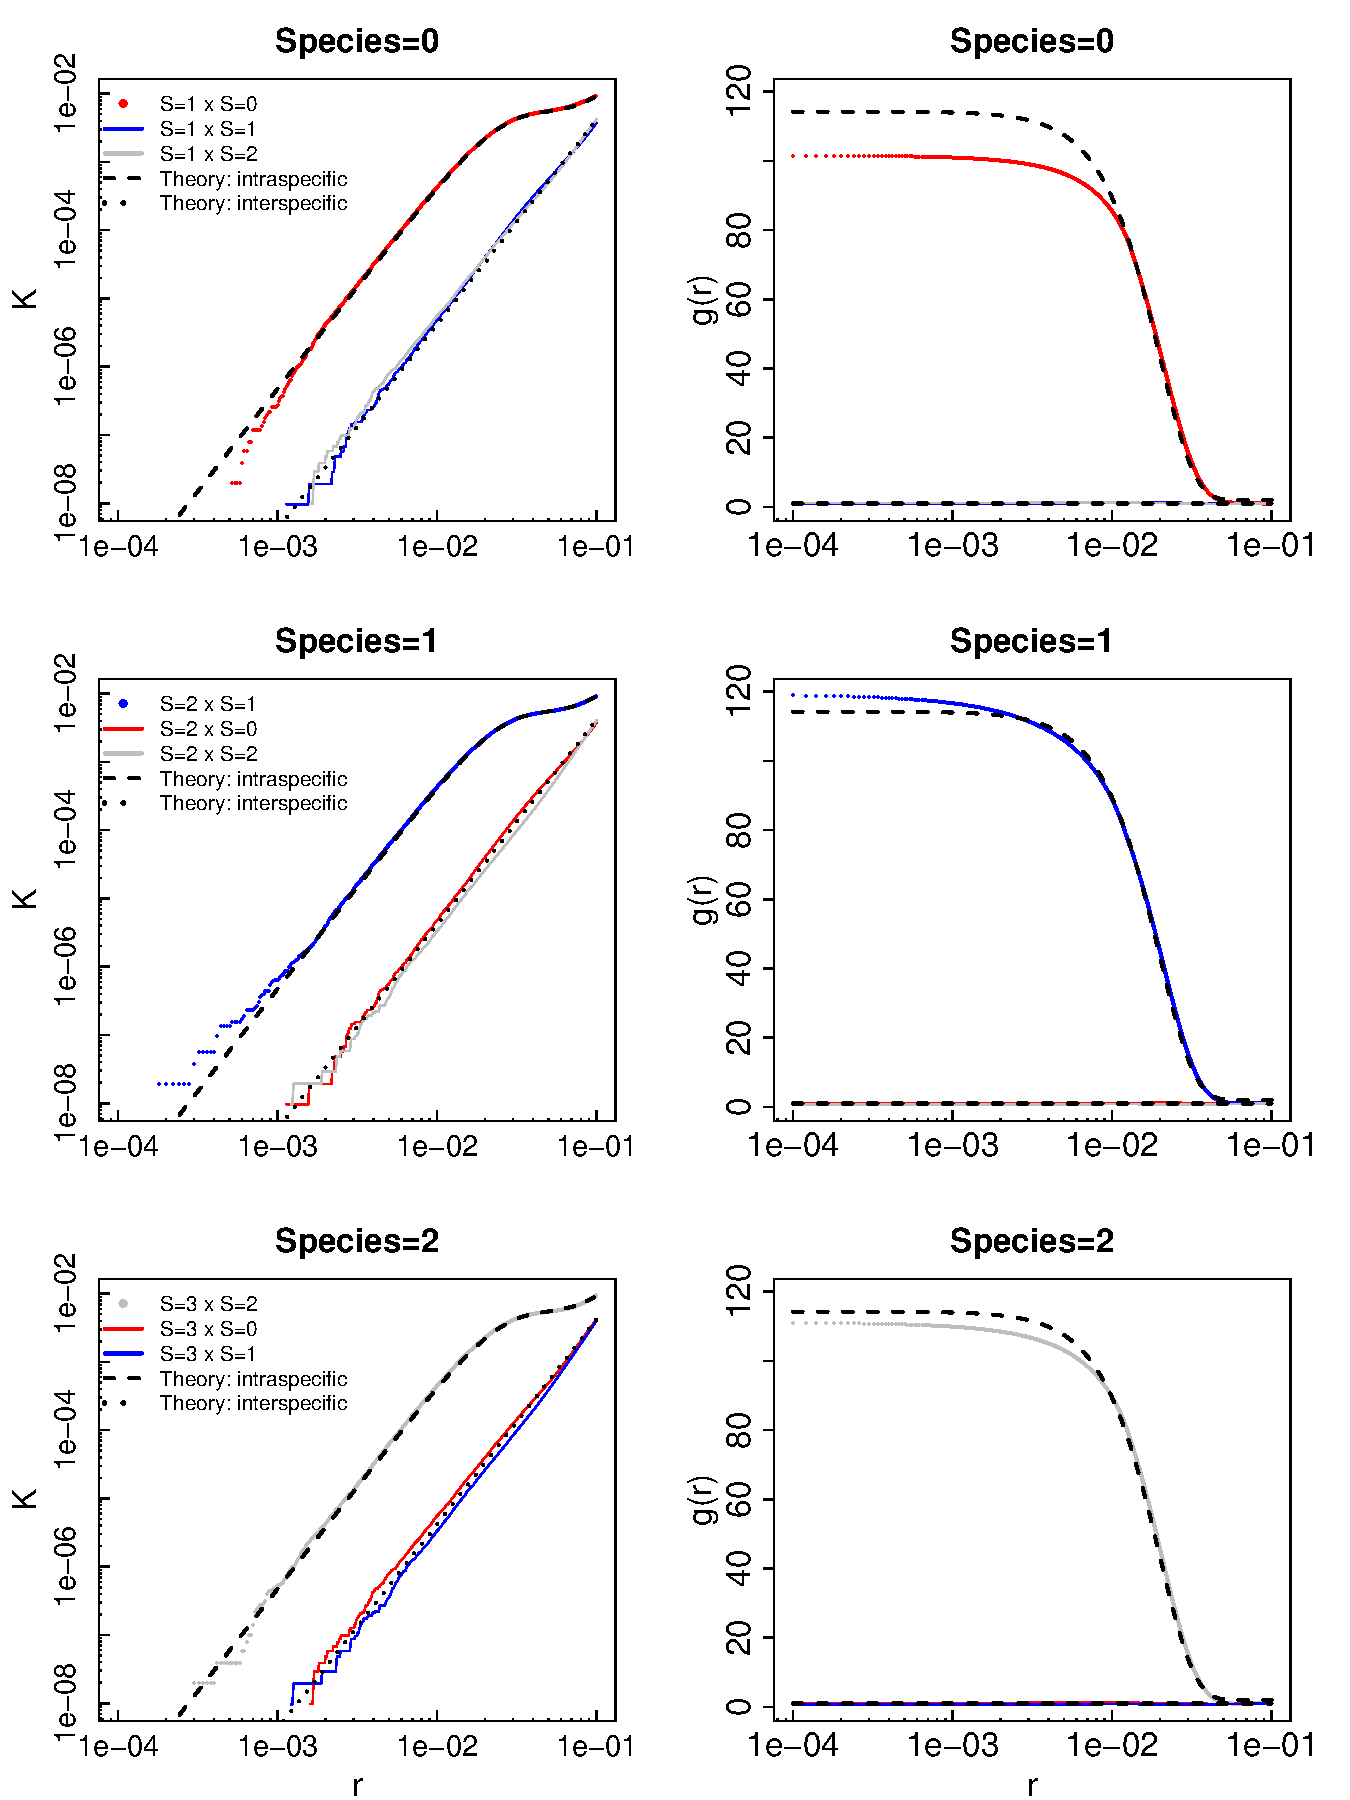
\includegraphics[width=0.8\textwidth]{../code/figure/K_PCF_Thomas}
\par\end{centering}
\caption{Intra- and inter-specific Ripley's $K$-function and pair correlation
function values as a function of distance (in cm) for 3 species following
a Thomas process with parent intensity $C_{p}=200$ cm$^{-3}$, number
of children per parent $N_{c}=50$, in a volume of 1 cm$^{3}$, $\sigma=0.01$
and $\delta\approx0.01$2. Values computed from our simulations (circles
and solid lines for intra- and interspecific values, respectively)
are compared with theoretical formula (dashed and dotted lines for
intra- and interspecific values, respectively). Colors correspond
to the different species (red for species 0, blue for species 1, black
for species 2). }
\end{figure}


\subsection{Brownian Bug Model}

While the pcf was one of the first indices that we intended to use,
we quickly realized that the combination of the large range of distances
we wanted to explore (from $10^{-4}$ to 1 cm) and the low density
of particles, at least for microphytoplankton, made the estimation
difficult as the choice of the bandwidth was critical. We give an
example of the sensitivity of the pcf computation to the bandwidth
below (Fig. \ref{fig:bandwidth_BBM}).

\begin{figure}[H]
\begin{centering}
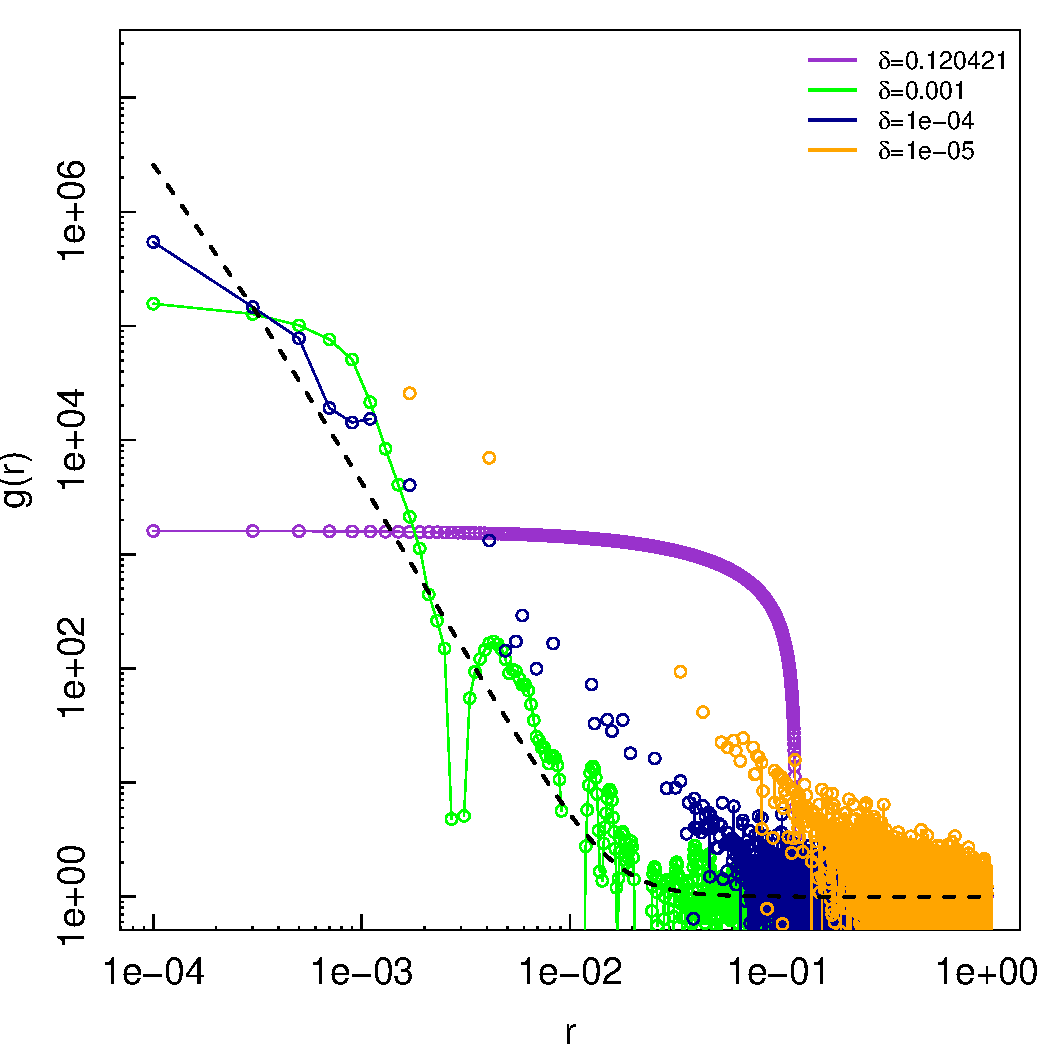
\includegraphics[width=0.6\textwidth]{../code/figure/bandwidth_BBM}
\par\end{centering}
\caption{Intraspecific pair correlation function as a function of distance
(in cm) computed for the Brownian bug model with microphytoplankton
particles, after 1000 time steps, with different values of the bandwidth
$\delta$. The dashed line indicates the theoretical pcf.\label{fig:bandwidth_BBM}
}
\end{figure}

We decided, from these results, to focus on Ripley's $K$-function,
which enabled us to compute the dominance index without having to
calibrate a bandwidth beforehand. 

\section{Spatial distributions}

\begin{figure}[H]
\begin{centering}
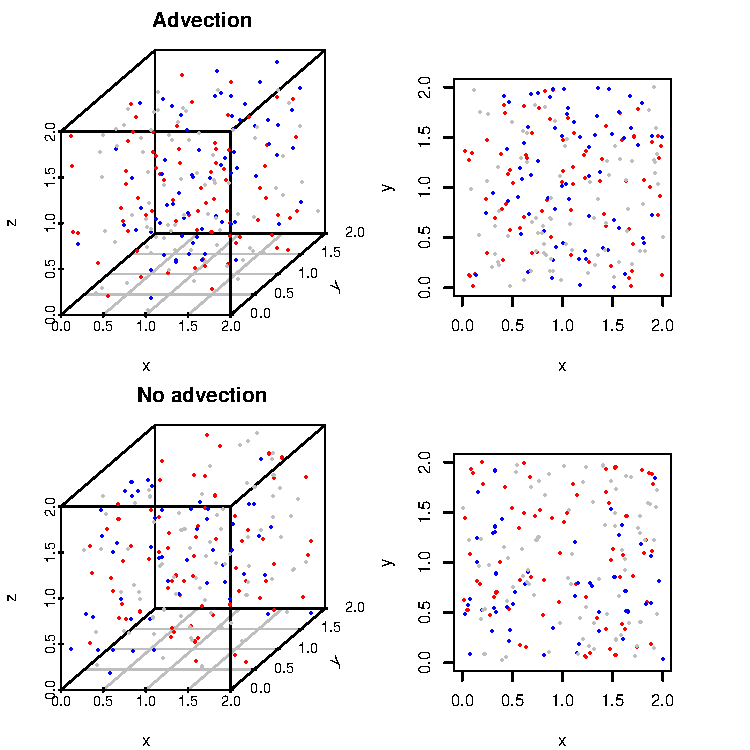
\includegraphics[width=0.99\textwidth]{../code/figure/spatial_distribution_zoom_micro0}
\par\end{centering}
\caption{Spatial distributions of a 3-species community of microphytoplankton
with and without advection with density $C=10$ cm$^{-3}$ after 1000
time steps. Each color corresponds to a different species. On the
left-hand side, only a zoom on a $2\times2\times2$ cm$^{3}$ cube
is shown, and its projection on the x-y plane is shown on the right
hand-side. \label{fig:Spatial-distributions} }
\end{figure}


\section{Minimum distances between points}

\subsubsection*{Theory}

One of the reasons why estimating $K$ and $g(r)$ is difficult is
that for small distances (below 10$^{-2}$), we can find very few
observations of pairs of points. As a first proxy, we want to estimate
the minimum expected distance between points (distance to the nearest
neighbour, DNN) when they are uniformly distributed.

\begin{doublespace}
In $d$ dimensions, the probability distribution of the distance $r$
to the nearest-neighbour follows $f(r)=db_{d}Cr^{d-1}\exp(-b_{d}r^{_{d}}C)$)
where $C$ is the intensity of the process. If we want to find the
distribution of the minimum DNN between $n$ realized points of a
Poisson process with intensity $C$, we can write:
\begin{equation}
\begin{array}{ccc}
\mathbb{P}(\min(R_{1},...,R_{n})>r) & = & \mathbb{P}(R_{1}>r,...,R_{n}>r)\\
 & = & \Pi_{i}^{n}\mathbb{P}(R_{i}>r)\\
 & = & \Pi_{i}^{n}\exp(-b_{d}r^{_{d}}C)\\
 & = & \exp(-b_{d}r^{_{d}}\Sigma_{i}^{n}C)
\end{array}
\end{equation}

\end{doublespace}

We can then conclude that the distribution of the minimum distance
follows the same distribution as the DNN, but with intensity $nC$.

\medskip{}

\citet{clark_generalization_1979} show that a variable with probability
distribution (with notations changed to fit our own) $f(r)=\frac{dC\pi^{d/2}r^{d-1}}{\Gamma(\frac{d}{2}+1)}\exp(-\frac{C\pi^{d/2}r^{d}}{\Gamma(\frac{d}{2}+1)})=dCb_{d}r^{d-1}\exp(-Cb_{d}r^{d})$
has an expected value of $\mu_{d}=\frac{\left(\Gamma(\frac{d}{2}+1)\right)^{1/d}\Gamma(\frac{1}{d}+1)}{C^{1/d}\pi^{1/2}}$.

With intensity $nC$, we can write $\frac{\left(\Gamma(\frac{d}{2}+1)\right)^{1/d}\Gamma(\frac{1}{d}+1)}{(nC)^{1/d}\pi^{1/2}}$.

\medskip{}

In 3D, 

\begin{doublespace}
\begin{equation}
\begin{array}{ccc}
\mu_{d} & = & (nC)^{-1/3}\frac{\left(\Gamma(\frac{3}{2}+1)\right)^{1/3}\Gamma(\frac{1}{3}+1)}{\pi^{1/2}}\\
 & = & (nC)^{-1/3}\left(\frac{3}{2}\Gamma(3/2)\right)^{1/3}\frac{1}{3}\Gamma(1/3)\frac{1}{\pi^{1/2}}\\
 & \approx & 0.554\frac{1}{(nC)^{1/3}}
\end{array}\label{eq:dnn_realization}
\end{equation}

\end{doublespace}

This needs to be taken into account when defining $C$. For microphytoplankton,
using $C=10$ cm$^{-3}$ and $n\approx10^{4}$, the smallest expected
distance for a uniform distribution is $1.2\times10^{-2}$ cm. For
nanophytoplankton, using $C=10^{3}$ cm$^{-3}$ and $n\approx10^{4}$,
it is reduced to $2.6\times10^{-3}$ cm. \medskip{}


\subsubsection*{Simulations}

We can compute the simulated distance to the nearest neighbour and
compare it to what we should obtain with a uniform distribution (Fig.
\ref{fig:Distance_micro} and \ref{fig:Distance_nano}): the simulated
average DNN are close to the expected value for a uniform distribution,
but the minimum distance to a conspecific is much lower than expected.

\begin{figure}[H]
\begin{centering}
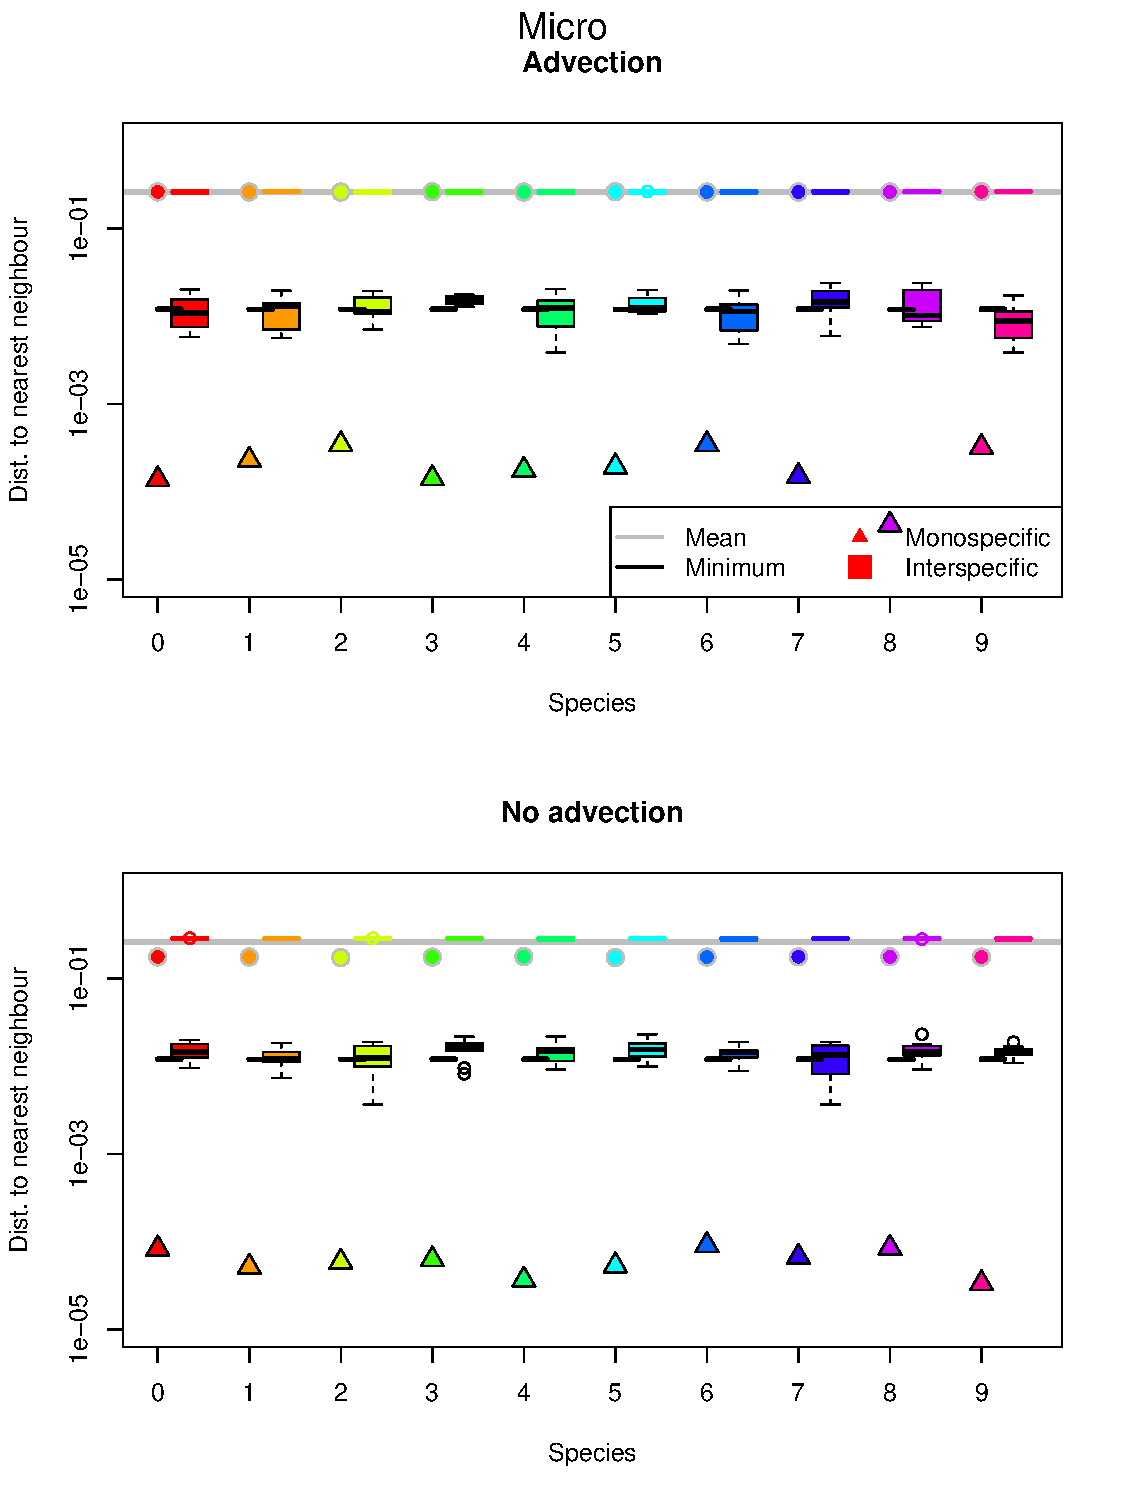
\includegraphics[width=0.7\textwidth]{../code/figure/distrib_distance_micro_box_10sp}
\par\end{centering}
\caption{Mean and minimum distance (in cm) to the nearest neighbour for 10
microphytoplankton species with density $C=10$ cm$^{-3}$, with and
without advection, after 1000 time steps, compared to predictions
for a uniform distribution. Horizontal lines show the average distance
to the nearest neighbour (grey line) and the expected minimum distance
to the nearest neighbour with the actual number of realizations (black
line). Circles and triangles represent mean and minimum distance to
a conspecific, respectively. Boxplot corresponds to the distribution
of mean (grey outlines) and minimum (black outlines) distances to
a heterospecific. Colors correspond to different species. \label{fig:Distance_micro}}
\end{figure}

\begin{figure}[H]
\begin{centering}
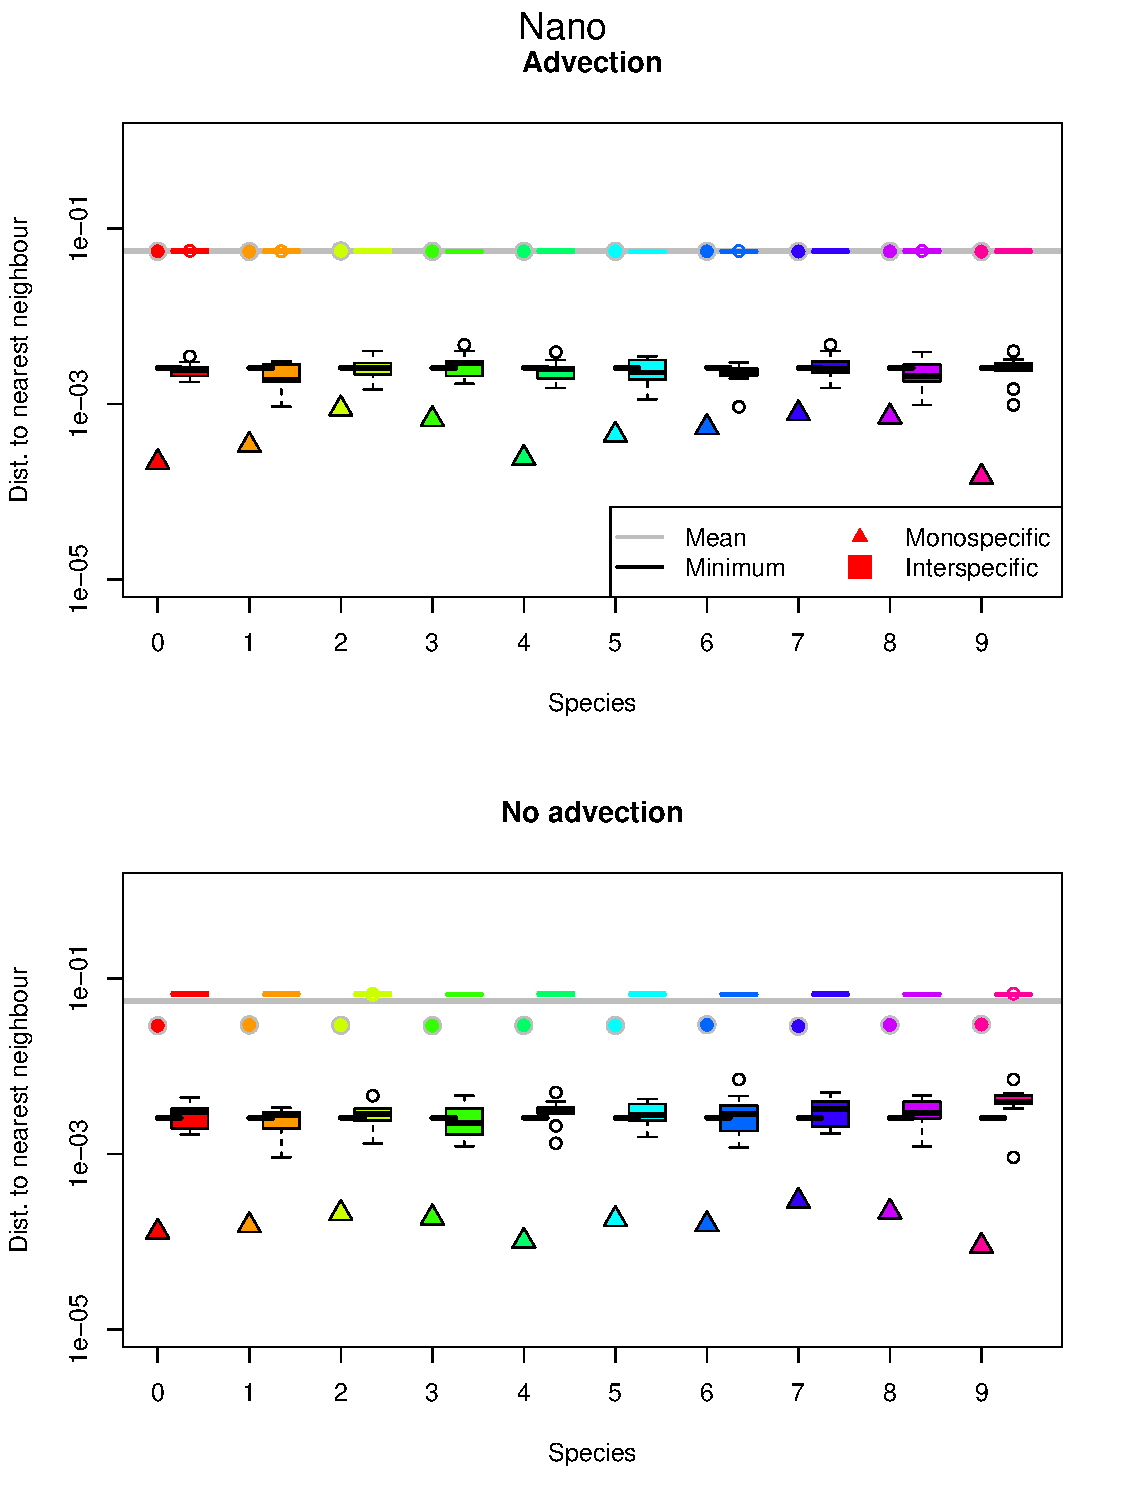
\includegraphics[width=0.7\textwidth]{../code/figure/distrib_distance_nano_box_10sp}
\par\end{centering}
\caption{Mean and minimum distance (in cm) to the nearest neighbour for 10
nanophytoplankton species with density $C=10^{3}$ cm$^{-3}$, with
and without advection, after 1000 time steps, compared to predictions
for a uniform distribution. Horizontal lines show the average distance
to the nearest neighbour (grey line) and the expected minimum distance
to the nearest neighbour with the actual number of realizations (black
line). Circles and triangles represent mean and minimum distance to
a conspecific, respectively. Boxplot corresponds to the distribution
of mean (grey outlines) and minimum (black outlines) distances to
a heterospecific. Colors correspond to different species. \label{fig:Distance_nano}}
\end{figure}


\subsubsection*{Relationship with densities}

In the case of a uniform distribution, an increase in density leads
to a decrease in distance to the nearest neighbour (eq. \ref{eq:dnn_realization}).
Mechanically, we can indeed expect that if the number of particles
increases within the same volume, they likely get closer to each other.
We confirm that this is also the case in the Brownian Bug Model. 

\begin{figure}[H]
\begin{centering}
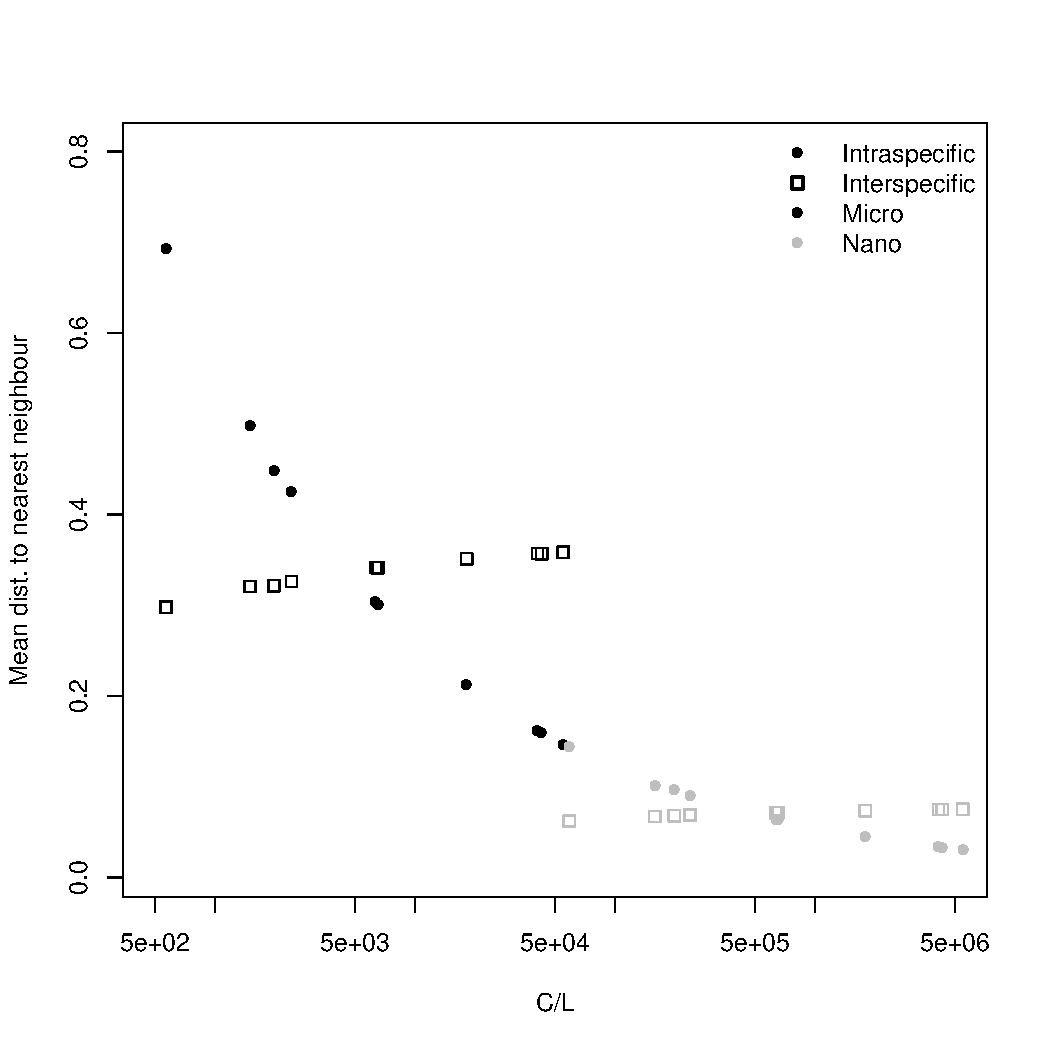
\includegraphics[width=0.75\textwidth]{../code/figure/dist_abundances_10sp_v2}
\par\end{centering}
\caption{Mean distance (in cm) to the nearest conspecific (filled circle) or
heterospecific (empty square) as a function of density in the environment
for both microphytoplankton (black) and nanophytoplankton (grey) communities
with a skewed abundance distribution, in the presence of advection.\label{fig:Distance_abundance}}
\end{figure}


\section{Effect of the initial distribution}

Particles are uniformly distributed in the cube at the start of all
simulations shown in the manuscript. However, we have no reason to
believe that such spatial distribution is more appropriate than a
more clustered one to begin with. In Fig. \ref{fig:Dominance-after_Thomas},
we show the final dominances obtained with and without advection,
starting from a superposition of Thomas processes, i.e. each species
was distributed with its own Thomas process. 

We need to modify the pair density function for the case without advection,
as the initial distribution changes from $G(r,0)=C^{2}$ to $G(r,0)=C^{2}+\frac{C^{2}}{C_{p}}\frac{1}{\left(4\pi\sigma^{2}\right)^{3/2}}e^{-\left(\frac{r^{2}}{4\sigma^{2}}\right)}$,
leading to eq. \ref{eq:K_bbm_thomas}.

\begin{equation}
K(r,t)=\frac{\lambda}{CD}\left(\frac{\rho^{2}}{2}-\frac{1}{2}\erf(\frac{\rho}{\sqrt{8Dt}})(\rho^{2}-4Dt)-\frac{\sqrt{2Dt}\rho}{\sqrt{\pi}}e^{-\rho^{2}/8Dt}\right)+\frac{4}{3}\pi r^{3}+\frac{1}{C_{p}\sigma\sqrt{\pi}}\left(\sigma\sqrt{\pi}\erf\left(\frac{r}{2\sigma}\right)-re^{-\left(\frac{r}{2\sigma}\right)^{2}}\right)\label{eq:K_bbm_thomas}
\end{equation}

\begin{figure}[H]
\begin{centering}
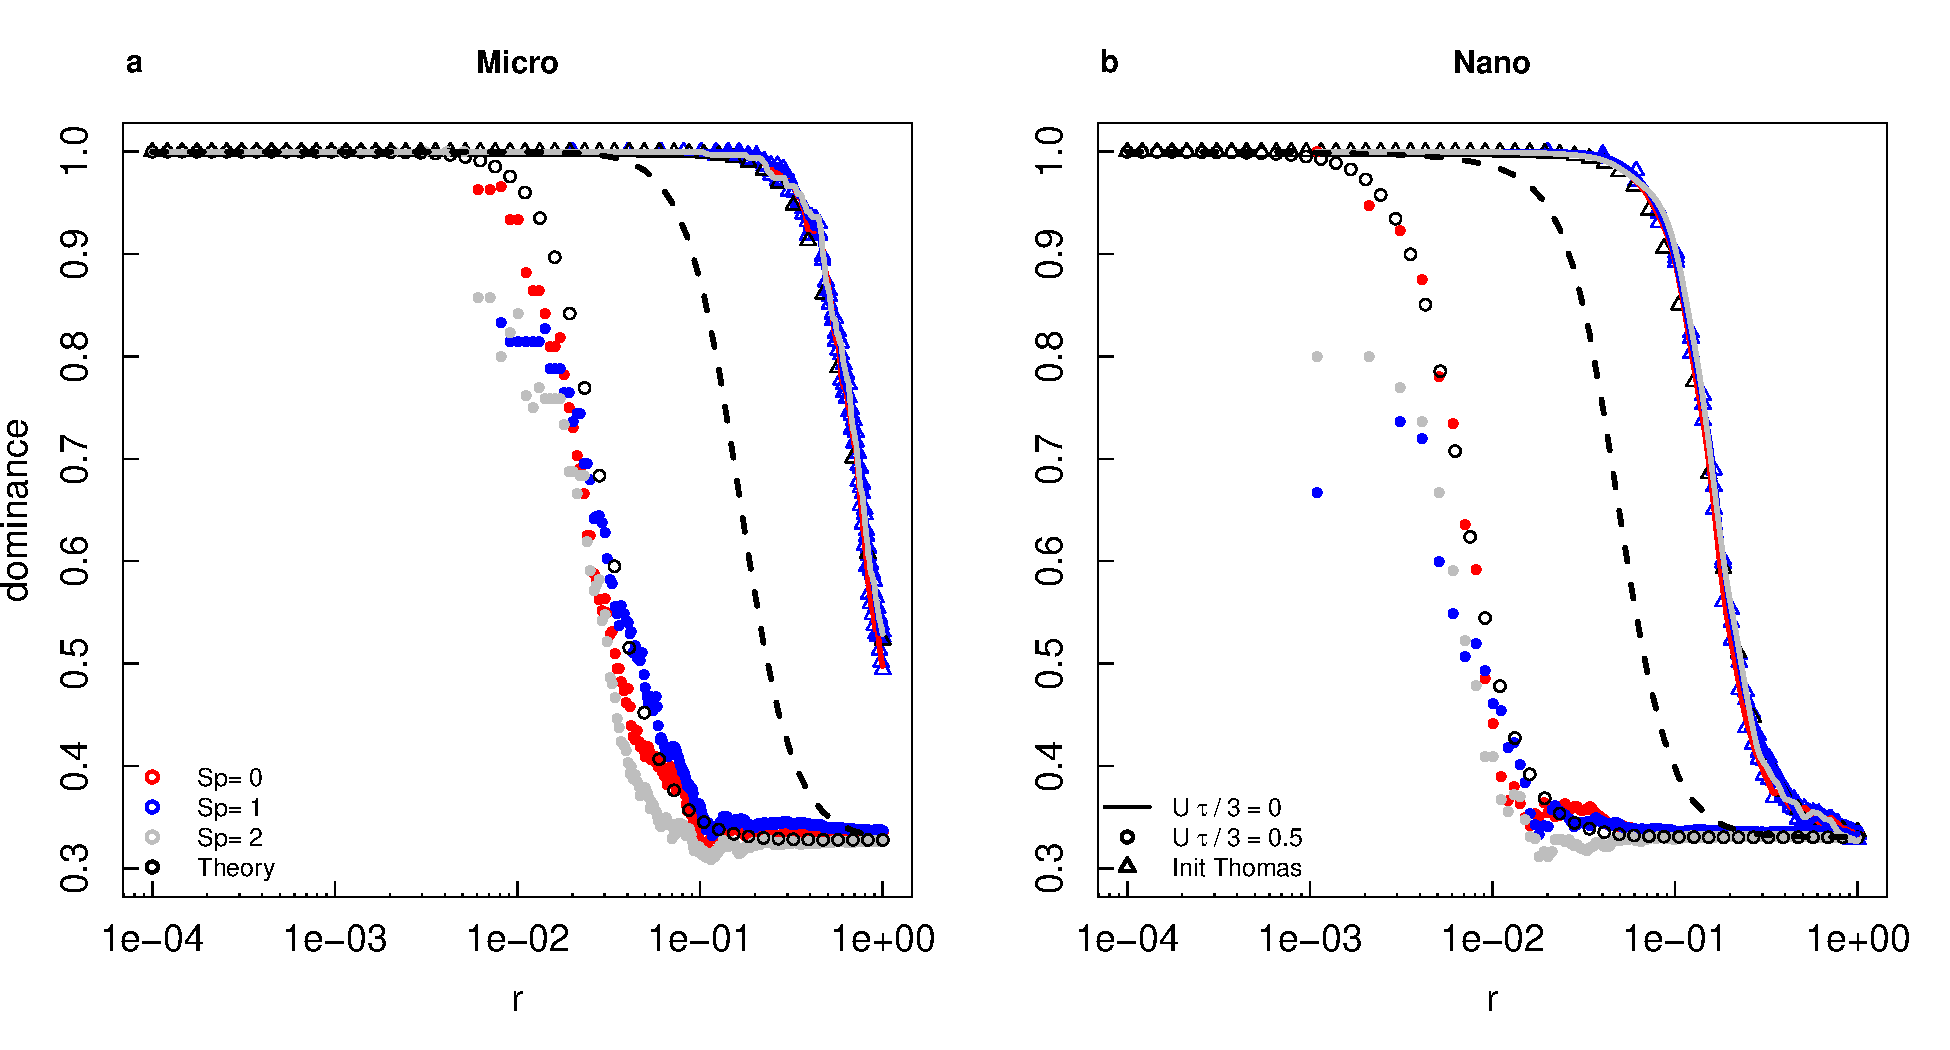
\includegraphics[width=0.95\textwidth]{../code/figure/shift_of_dominance}
\par\end{centering}
\caption{Dominance indices as a function of distance (in cm) for microphytoplankton
(a) and nanophytoplankton (b) in a 3-species community with even distributions
after 1000 timesteps starting from a superposition of species-specific
Thomas point processes, with (circles) and without (lines) advection.
The triangles correspond to the dominance index at the start of the
simulation, i.e. when points are only distributed according to a Thomas
point process with parent intensity $C_{p}=200$ cm$^{-3}$, number
of children per parent $N_{c}=50$, and $\sigma=0.001$. Each color
represents a different species. The black points and line corresponds
to the theoretical values of the dominance index.\label{fig:Dominance-after_Thomas}}

\end{figure}

Simulated and theoretical values match for a 1000-time steps duration
(Fig. \ref{fig:Dominance-noadv_Thomas}). .

\begin{figure}[H]
\begin{centering}
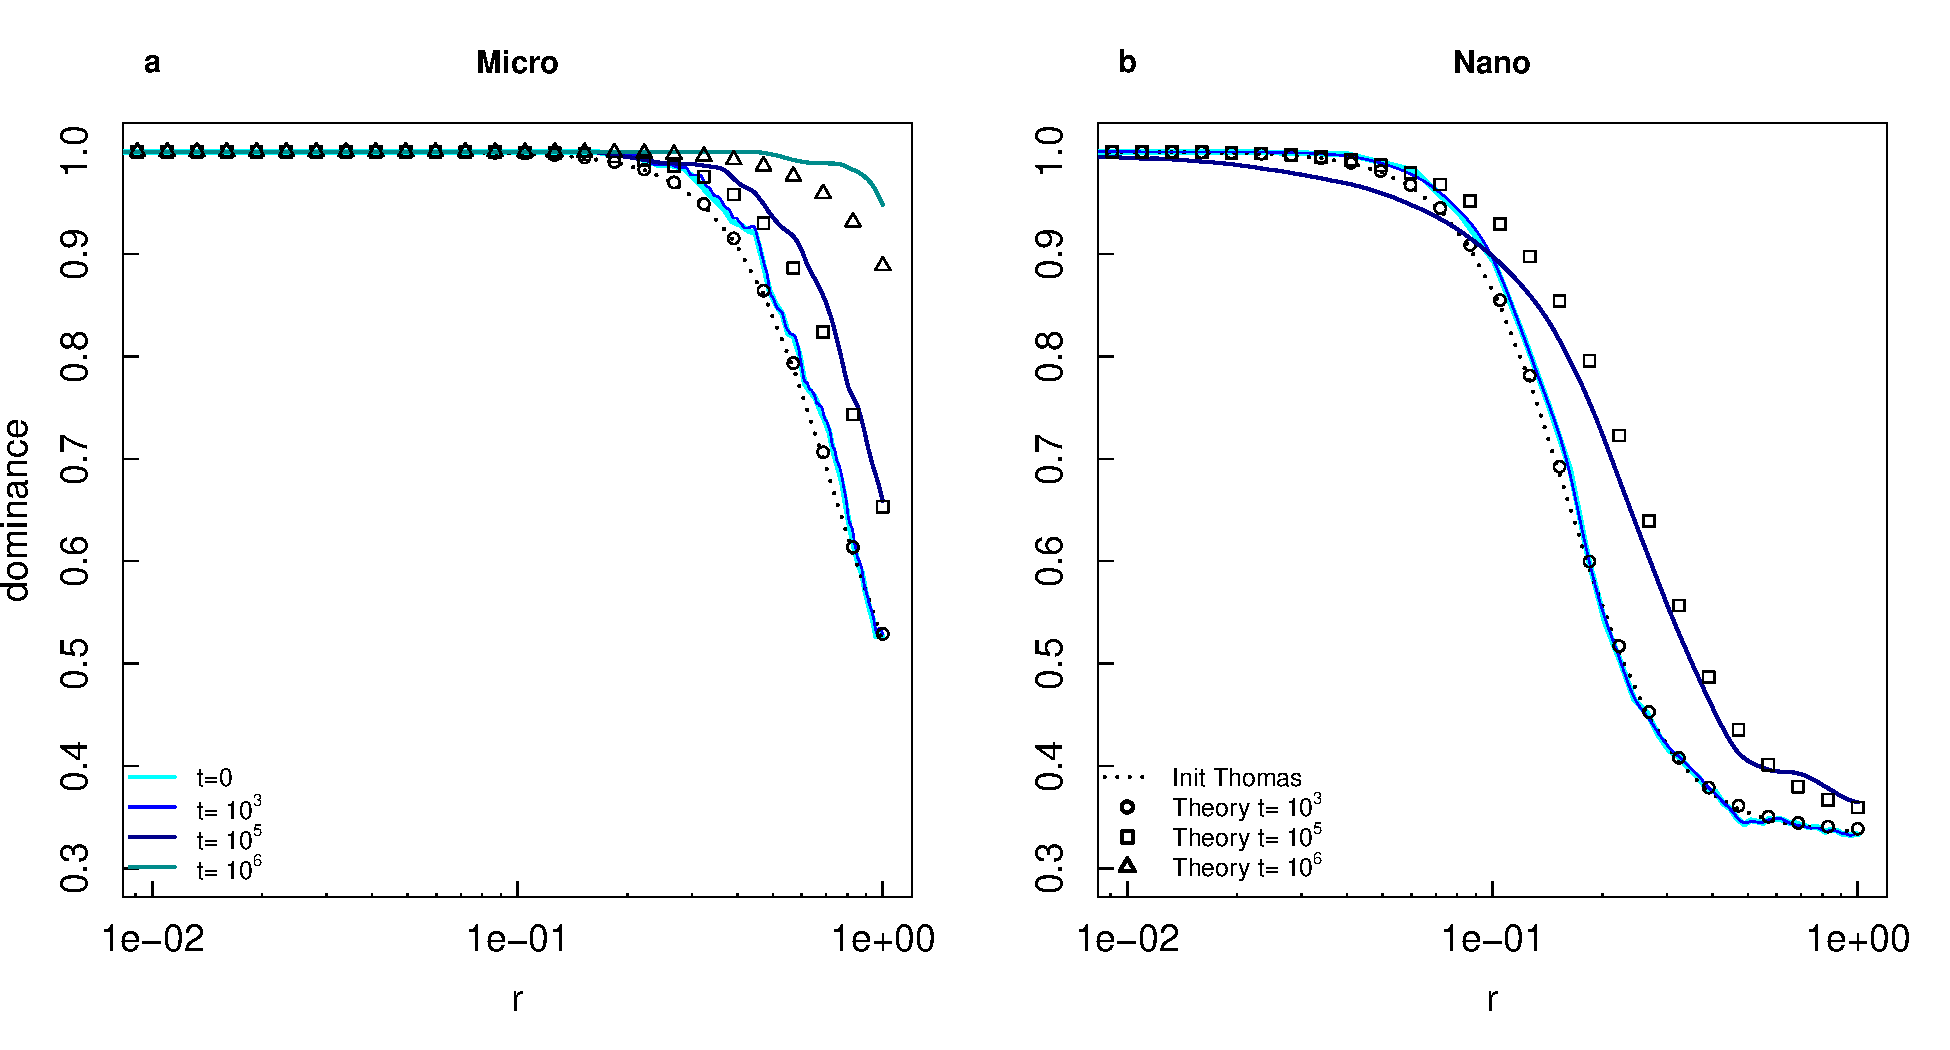
\includegraphics[width=0.95\textwidth]{../code/figure/shift_of_dominance_noadv_zoom}
\par\end{centering}
\caption{Dominance indices as a function of distance (in cm) for one species
in a microphytoplankton (a) and nanophytoplankton (b) 3-species community
with even distributions after 1000 timesteps starting from a superposition
of species-specific Thomas point processes in the absence of advection.
The dotted line corresponds to the dominance index at the start of
the simulation, i.e. when points are only distributed according to
a Thomas point process with parent intensity $C_{p}=200$ cm$^{-3}$,
number of children per parent $N_{c}=50$, and $\sigma=0.001$. Each
colored line represents a different simulation duration, and black
symbols correspond to the theoretical values of the dominance index.\label{fig:Dominance-noadv_Thomas}}
\end{figure}


\section{Sensitivity to the computation of the advection parameter}

If we we define a length $L_{v}$ corresponding to the equivalent
sphere diameter, i.e.:

\begin{equation}
\begin{array}{cccc}
 & \frac{4}{3}\pi\left(\frac{L_{v}}{2}\right)^{3} & = & L_{c}^{3}\\
\Leftrightarrow & L_{v} & = & 2L_{c}\left(\frac{3}{4\pi}\right)^{1/3}\\
\Leftrightarrow & L_{v} & = & 1.24\text{ cm}
\end{array}\label{eq:re_lv}
\end{equation}
If we use $U\approx\nu/L_{v}$, $U\approx8.1\times10^{-5}$ m.s$^{-1}$.
Using $U\tau/3=0.5$ cm, we have $\tau=185\text{ s}=2.1\times10^{-3}$
d. This means that $\gamma=164$. As could be expected, when the flow
velocity decreases, mixing decreases (Fig. \ref{fig:Dominance_advection}).

\begin{figure}[H]
\begin{centering}
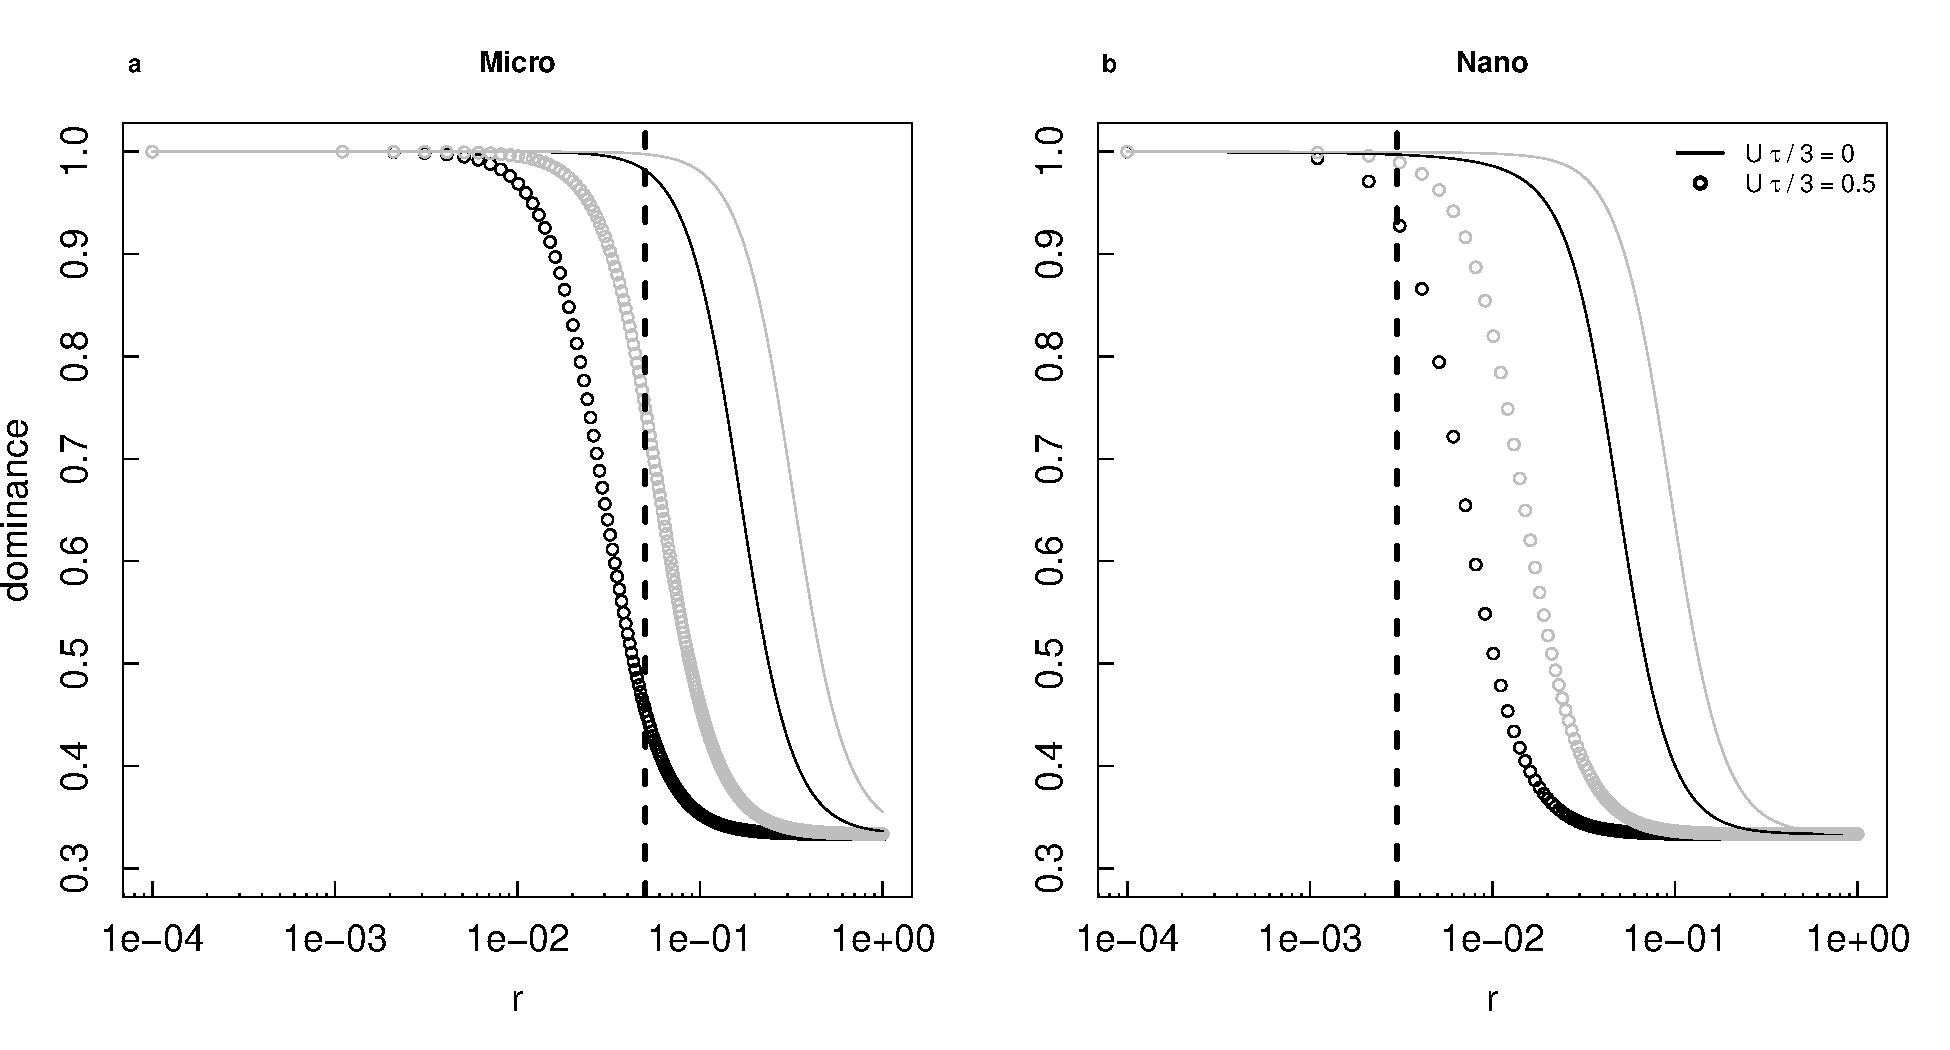
\includegraphics[width=0.99\textwidth]{../code/figure/theoretical_dominance_with_adv}
\par\end{centering}
\caption{Dominance indices as a function of distance (in cm) for one species
in a microphytoplankton (a) and nanophytoplankton (b) 3-species community
with even distributions after 1000 timesteps with (circles) and without
(lines) advection for different duration of the timesteps, with reference
parameters (black) and lower flow velocity (grey). \label{fig:Dominance_advection}}

\end{figure}

\bibliographystyle{ecol_let}
\bibliography{bibliography}

\end{document}
